%!TEX root = ../main.tex

\chapter{Data Model}
\label{ch:data_model}

Das Data Model von \textit{Soli} ist in die Pakete \textit{dto} und \textit{domain} aufgeteilt.
Die \textit{dto}-Klassen sind die Datenübertragungsobjekte, die die Daten zwischen den Schichten des Systems übertragen.
Die \textit{domain}-Klassen sind die Datenobjekte, die in der Datenbank gespeichert werden, und bilden somit das interne Datenmodell des Systems.

Dieses Datenmodell wird mithilfe von \gls{SpringData} in der \gls{PostgreSQL}-Datenbank (welche sich zur Isolation in einem separaten \gls{Container} befindet) abgebildet.
In dieser wird das Datenmodell in Form von Tabellen und Beziehungen zwischen diesen gespeichert.
In der Anwendung werden die Datenobjekte nur im Kontext aktiver Anfragen im Arbeitsspeicher gehalten und bei Bedarf in die Datenbank geschrieben.
Als Konsequenz können die \gls{ACID}-Eigenschaften der Datenbank genutzt werden, um die Daten vor Verlust oder Inkonsistenzen zu schützen.
Damit die Daten auch über zukünftige Aktualisierungen des Systems hinweg erhalten bleiben, wird das Datenbankmigrationssystem \gls{Flyway} genutzt, das die Datenbankstruktur anpasst, wenn sich das Datenmodell ändert.

Den Kern des Buchungsmodells bildet die Klasse \hyperref[edu.kit.hci.soli.domain.Booking]{\texttt{Booking}}, die eine Buchung eines Raumes repräsentiert.
Jede Buchung ist einem Raum und einem Nutzer zugeordnet und hat einen Start- und Endzeitpunkt.
Außerdem kann eine Buchung optional einen Kommentar enthalten, der von dem Nutzer hinterlassen wurde.
Zur Umsetzung von Buchungen des Kooperationstyps \textit{ON\_REQUEST} existiert zudem eine automatisch verwaltete Tabelle von noch offenen Anfragen für eine Buchung.

Da die Authentifikation von Nutzenden nicht durch das System selbst, sondern durch das \gls{OIDC}-System des KIT erfolgt, werden statt vollen Anmeldedaten nur die OIDC-IDs der Nutzenden gespeichert.
Diese sind im \hyperref[edu.kit.hci.soli.domain.User]{\texttt{User}}-Objekt unter dem Namen \texttt{userId} mit dem Präfix \texttt{kit/} abgelegt.
Gäste erhalten eine interne ID, welche mit dem Präfix \texttt{guest/} beginnt, und somit von den IDs der KIT-Nutzenden unterschieden werden kann.
Der Administrator des Systems hat die fixe interne ID \texttt{admin}.
Die Tabelle der Nutzenden ergänzt diese Information um die E-Mail-Adresse, den Namen und die Sprache der Nutzenden, welche für die Kommunikation mit diesen (z.B. per E-Mail) genutzt werden.
Außerdem wird eine Flagge gespeichert, die es Administratoren ermöglicht, einzelne Nutzende zu sperren.

Eine Raumtabelle wird genutzt, um die Erweiterbarkeit des Systems zu gewährleisten.
In dieser Tabelle wird im minimalen System entsprechend den Musskriterien nur ein Raum gespeichert, welcher die ID \texttt{1} trägt.

Eine Übersicht des Datenbankmodells ist in \autoref{fig:data_model} dargestellt.

\begin{figure}[ht]
    \centering
    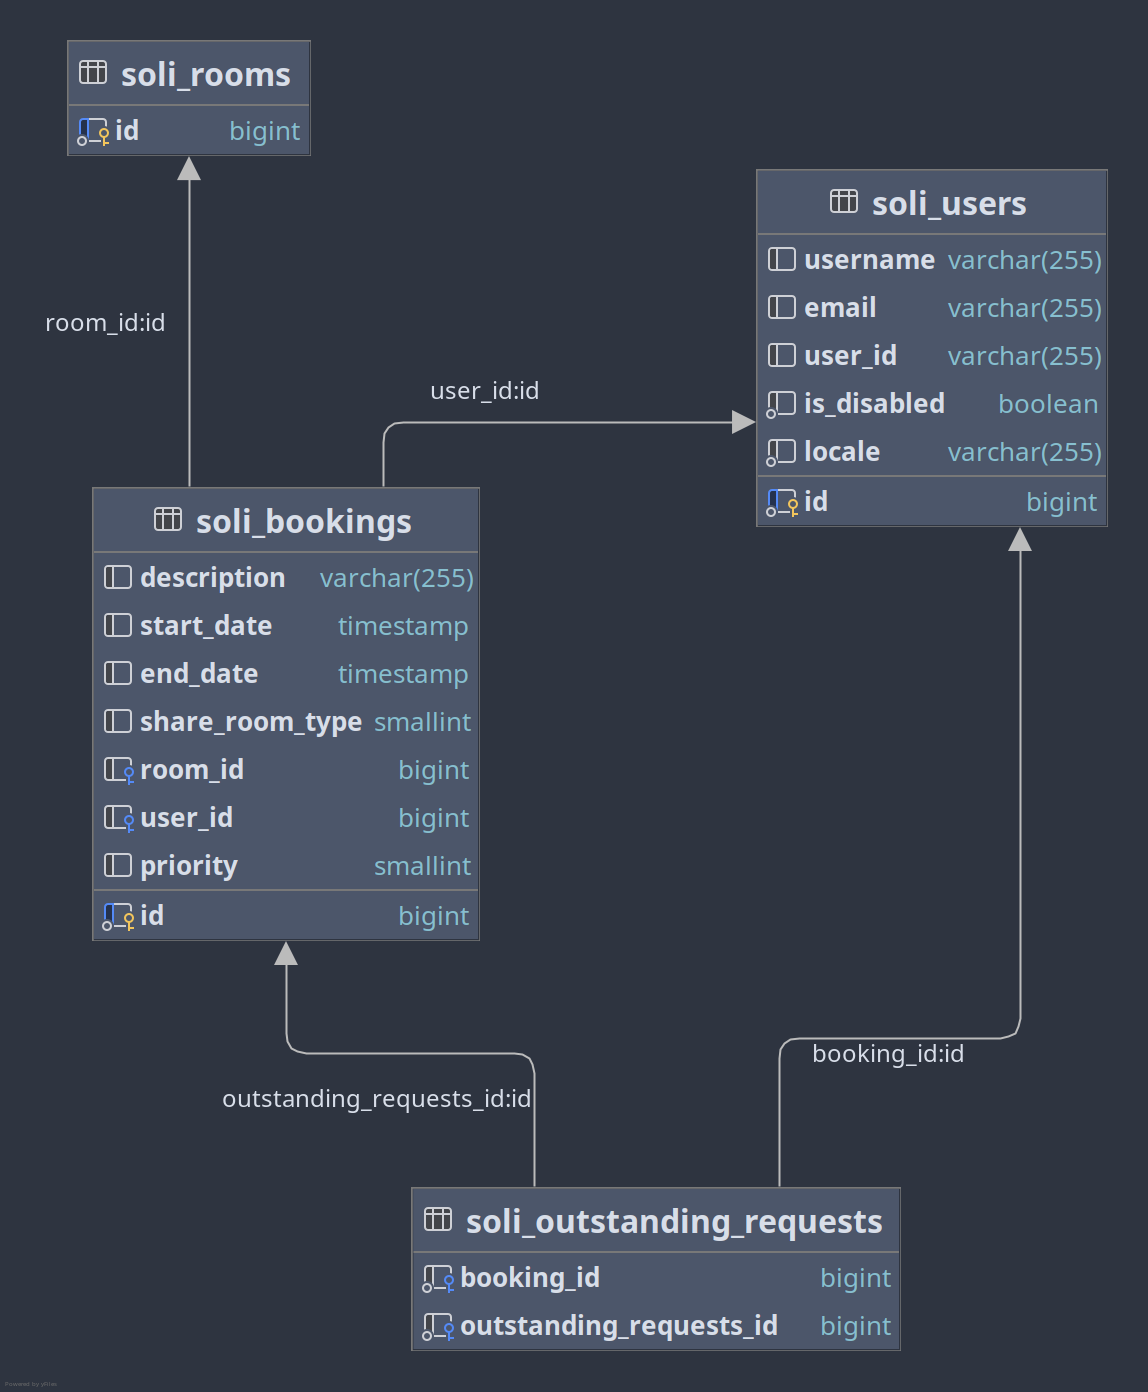
\includegraphics[width=\textwidth]{figures/database}
    \caption{Datenbankmodell von \textit{Soli}}
    \label{fig:data_model}
\end{figure}
\pagebreak

\InputIfFileExists{javadoc/edu.kit.hci.soli.dto}{}{}
\InputIfFileExists{javadoc/edu.kit.hci.soli.domain}{}{}
